\documentclass[paper=a4, fontsize=10pt]{scrartcl}
\usepackage[bottom=1in, left=1in, right=1in, top=1in]{geometry}
\usepackage{layouts}

\usepackage[usenames,dvipsnames,x11names]{xcolor}

\usepackage[T1]{fontenc}
\usepackage{fourier}
\usepackage[english]{babel}
\usepackage{amsmath,amsfonts,amsthm}

\usepackage{sectsty}
\allsectionsfont{\centering \normalfont\scshape}

\usepackage{tikz}
\usepackage{pgfplots}
\usetikzlibrary{plotmarks}

\usepackage{booktabs}
\usepackage{longtable}
\usepackage{tabularx}
\usepackage{ragged2e}
\newcolumntype{Y}{>{\RaggedRight\arraybackslash}X}
\usepackage{paralist}

\usepackage{acronym}
\usepackage[inline]{enumitem}
\usepackage{fancyhdr}
\usepackage{graphicx}
\usepackage{lastpage}
\usepackage{listings}
\usepackage{multirow}
\usepackage{subfigure}
\usepackage[htt]{hyphenat}

\pagestyle{fancyplain}
\fancyhead{}
\fancyfoot[L]{}
\fancyfoot[C]{\thepage~of~4}
\renewcommand{\headrulewidth}{0pt}
\renewcommand{\footrulewidth}{0pt}
\setlength{\headheight}{13.6pt}

\newcommand{\horrule}[1]{\rule{\linewidth}{#1}}

% For code fragments:
%\usepackage{fontspec}
\usepackage{minted}
%\setsansfont{Calibri}
%\setmonofont{Consolas}

\usepackage{algorithm, algpseudocode}
\usepackage{caption}
\usepackage{float}
\usepackage{tabu}

\usepackage{hyperref}
\hypersetup{hidelinks}

\pgfplotsset{compat=1.5}
\usepackage{pgfplots, pgfplotstable}
\usepgfplotslibrary{colorbrewer}
\usepgfplotslibrary{fillbetween}

\pgfplotsset{
every axis/.append style={
scale only axis,
width=0.40\textwidth,height=0.3\textwidth,
},
/tikz/every picture/.append style={
trim axis left,
trim axis right,
baseline
}
}

% http://tex.stackexchange.com/questions/67895/is-there-an-easy-way-of-using-line-thickness-as-error-indicator-in-a-plot

% Takes six arguments: data table name, x column, y column, error column,
% color and error bar opacity.
% ---
% Creates invisible plots for the upper and lower boundaries of the error,
% and names them. Then uses fill between to fill between the named upper and
% lower error boundaries. All these plots are forgotten so that they are not
% included in the legend. Finally, plots the y column above the error band.
\newcommand{\errorband}[6]{
\pgfplotstableread{#1}\datatable
  \addplot [name path=pluserror,draw=none,no markers,forget plot]
    table [x={#2},y expr=\thisrow{#3}+\thisrow{#4}] {\datatable};

  \addplot [name path=minuserror,draw=none,no markers,forget plot]
    table [x={#2},y expr=\thisrow{#3}-\thisrow{#4}] {\datatable};

  \addplot [forget plot,fill=#5,opacity=#6]
    fill between[on layer={},of=pluserror and minuserror];

  \addplot [#5,thick,no markers]
    table [x={#2},y={#3}] {\datatable};
}


\title{
\normalfont \normalsize
\textsc{Norwegian University of Science and Technology\\IT3708 -- Bio-Inspired Artificial Intelligence}
\horrule{0.5pt} \\[0.4cm]
\huge Project 1:\\ Supervised and Reinforcement Learning of\\Neural Agent Controllers\\
\horrule{2pt} \\[0.5cm]
}

\author{Per Magnus Veierland\\permve@stud.ntnu.no}

\date{\normalsize\today}

\begin{document}

%\fancyfoot[C]{}
\maketitle

\section*{Implementation and Baseline}

The assignment program is a single file \texttt{program.py} written in Python programming language using the NumPy library for computation. PyQt bindings are used to render vector visualizations to PDF. The visualization uses an \textsc{X} to mark the agent starting point, and an increasing line thickness to indicate the direction of movement. The most important classes are the \texttt{BaselineAgent}, \texttt{SupervisedLearningAgent}, and \texttt{ReinforcementLearningAgent}, which implement the method \texttt{act(percepts)} which returns a \texttt{FlatlandAction}. The \texttt{percepts} parameter is a $(3,S)$ N-dimensional array, where the first dimension is the direction, and the second is the sensor range ($S$).

\begin{figure}
\centering
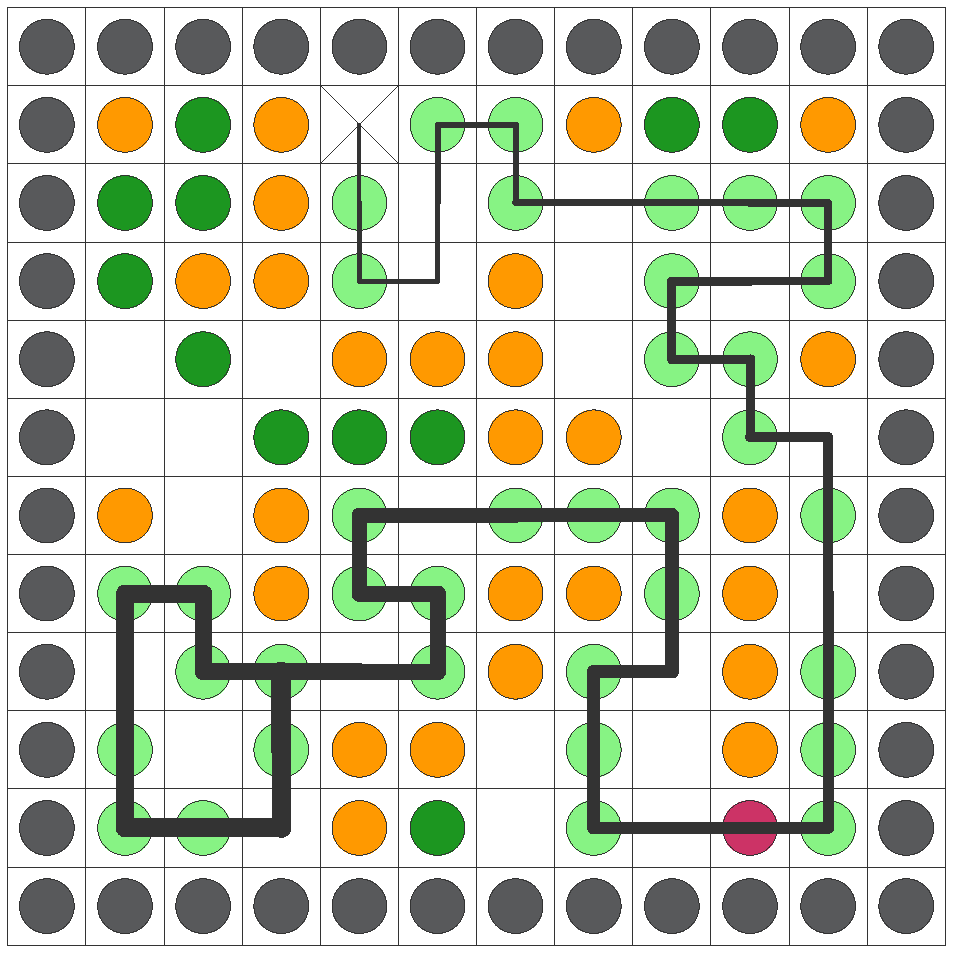
\includegraphics[scale=0.2]{../data/render-baseline.pdf}
\caption{Flatland visualization of baseline agent}
\label{figure:flatland_baseline}
\end{figure}

The baseline agent's behavior is to always move towards food. If there is no neighboring food, it will move towards an open location. If there are no open locations it will move towards poison. Given how the world is defined the baseline agent will never need to move into obstacles. If there are more than one possible destination of the same kind, it will prefer moving forward, otherwise left, otherwise right, accordingly.

The mean score achieved by the baseline agent is $20.2$ averaged over 1~million~trials.

\section*{Supervised Learning Agent}

Computation of the delta values used for updating weights is shown in Figure~\ref{fig:code_delta_supervised}. The \textit{CorrectChoice} is a \textit{one-hot encoded} vector where the index of the target action is set to 1. To make the softmax computation numerically stable we use the reformulation described in Equation~\ref{eq:softmax} with $\log C = -\max y_j$, such that the greatest exponent factor is 0.

\begin{equation}
\frac{e^{y_j}}{\sum_k e^{y_k}} = \frac{C \cdot e^{y_j}}{C \cdot \sum_k e^{y_k}} = \frac{e^{y_j + \log C}}{\sum_k e^{y_k + \log C}}
\label{eq:softmax}
\end{equation}

% TODO Plot how your agent’s performance develops as the number of training rounds increases. The score value plotted for a given training round should be the average score over all of the Flatland worlds trained on during that round (which should be a large number of Flatland worlds such as 100).

\begin{figure}[H]
\footnotesize
\begin{minted}[mathescape,
               linenos,
               numbersep=5pt,
               frame=lines,
               framesep=2mm]{python}
def train(self, percepts, target_action, learning_rate):
  inputs   = encode_percepts(percepts)
  outputs  = np.dot(self.weights, inputs)
  outputs -= np.max(outputs) # Shift values for softmax numerical stability
  softmax  = np.exp(outputs) / np.sum(np.exp(outputs))
  correct_choice = np.zeros(3)
  correct_choice[target_action] = 1 
  delta = correct_choice - softmax
  self.weights += learning_rate * np.dot(delta.reshape((3, 1)), inputs.reshape((1, 12)))
\end{minted}
\vspace*{-5mm}
\caption{\textit{Widroff-Hoff} rule implementation with cross-entropy ``softmax'' loss.}
\label{fig:code_delta_supervised}
\end{figure}

\begin{figure}[H]
\centering
\begin{tabularx}{\textwidth}{XcXc}
~ &
\begin{tikzpicture}
\begin{axis}[xlabel={Generations},ylabel={Fitness / time step}]
\errorband{../data/learning-curve-supervised-25-training-rounds-10-average.txt}{0}{1}{2}{Cyan}{0.4}
\end{axis}
\end{tikzpicture}
& ~ &
\begin{tikzpicture}
\begin{axis}[xlabel={Generations},ylabel={Fitness / time step}]
\errorband{../data/learning-curve-supervised-25-training-rounds-10-average.txt}{0}{1}{2}{Cyan}{0.4}
\end{axis}
\end{tikzpicture}
\\
\end{tabularx}
\caption{\ac{EANN} performance when trained on 1~static~scenario~(left), and on 5~static~scenarios~(right). Mean population fitness is shown in blue with standard deviation shown in light blue, and the fitness of the best individual is shown in red.}
\label{fig:performance_static}
\end{figure}

\section*{Reinforcement Learning Agent}

\begin{figure}[H]
\footnotesize
\begin{minted}[mathescape,
               linenos,
               numbersep=5pt,
               frame=lines,
               framesep=2mm]{python}
def train(self, percepts, percepts_next, learning_rate, discount_factor, reward):
  inputs, outputs = self.evaluate(percepts)
  action          = np.argmax(outputs)
  q_current       = outputs[action]
  q_next          = np.amax(self.evaluate(percepts_next)[1])
  delta           = (encode_int_as_one_hot(action, 3) *
                    (reward + discount_factor * q_next - q_current))
  self.update_weights(learning_rate, delta, inputs)
\end{minted}
\vspace*{-5mm}
\caption{\textit{Widroff-Hoff} rule implementation with cross-entropy ``softmax'' loss.}
\label{fig:code_delta_reinforcement}
\end{figure}



\begin{table}
\footnotesize
\begin{tabular}{*{13}{c@{\hskip 1.8mm}}}
\toprule
Action & \textsc{LE} & \textsc{LW} & \textsc{LF} & \textsc{LP} & \textsc{FE} & \textsc{FW} & \textsc{FF} & \textsc{FP} & \textsc{RE} & \textsc{RW} & \textsc{RF} & \textsc{RP} \\
\midrule
\textsc{Left} & \textsc{2.05196} & \textsc{-2.96582} & \textsc{3.70593} & \textsc{-1.49711} & \textsc{0.76775} & \textsc{0.44683} & \textsc{-0.83441} & \textsc{0.91687} & \textsc{0.22473} & \textsc{0.41743} & \textsc{0.31837} & \textsc{0.33445} \\
\textsc{Forward} & \textsc{0.49009} & \textsc{0.41783} & \textsc{0.44274} & \textsc{0.51937} & \textsc{2.39228} & \textsc{-2.97048} & \textsc{3.74041} & \textsc{-1.29415} & \textsc{0.57521} & \textsc{0.03054} & \textsc{0.63301} & \textsc{0.63222} \\
\textsc{Right} & \textsc{0.68777} & \textsc{0.94304} & \textsc{-1.00009} & \textsc{0.91515} & \textsc{0.47364} & \textsc{0.07497} & \textsc{0.50149} & \textsc{0.49892} & \textsc{1.96840} & \textsc{-1.99461} & \textsc{3.35978} & \textsc{-1.78186} \\
\bottomrule
\end{tabular}
\caption{Weights for trained reinforcement learning agent with sensor range of 1.}
\label{table:weights}
\end{table}

\end{document}

